\documentclass[aspectratio=169]{beamer}

\usetheme{Boadilla}
\usefonttheme{professionalfonts}
\setbeamertemplate{navigation symbols}{}
\setbeamertemplate{itemize items}[circle]
\setbeamertemplate{enumerate items}[default]
\setbeamertemplate{headline}{}

\usepackage[utf8]{inputenc}
\usepackage[T1]{fontenc}
\usepackage{lmodern}
\usepackage{amsmath}
\usepackage{booktabs}
\usepackage{tabularx}
\usepackage{array}
\usepackage{hyperref}
\usepackage[strings]{underscore}
\usepackage{listings}
\usepackage{tikz}
\usetikzlibrary{arrows.meta,positioning,fit,calc,shapes.geometric}
\usepackage{xcolor}

\definecolor{courseblue}{HTML}{12355B}
\definecolor{coursegold}{HTML}{C98A2E}
\definecolor{courseice}{HTML}{EEF3F8}
\definecolor{coursegreen}{HTML}{2F6B4F}
\definecolor{coursegray}{HTML}{4B5563}
\definecolor{codebg}{HTML}{F7F9FC}
\definecolor{codecomment}{HTML}{5E6C84}
\definecolor{codestring}{HTML}{0B6E4F}

\setbeamercolor{palette primary}{bg=courseblue,fg=white}
\setbeamercolor{palette secondary}{bg=coursegold,fg=white}
\setbeamercolor{palette tertiary}{bg=courseblue,fg=white}
\setbeamercolor{palette quaternary}{bg=coursegold,fg=white}
\setbeamercolor{structure}{fg=courseblue}
\setbeamercolor{frametitle}{bg=courseice,fg=courseblue}
\setbeamercolor{title}{fg=courseblue}
\setbeamercolor{block title}{bg=courseblue,fg=white}
\setbeamercolor{block body}{bg=courseice,fg=black}
\setbeamercolor{normal text}{fg=black,bg=white}
\setbeamercolor{alerted text}{fg=coursegold}

\setbeamerfont{footline}{size=\scriptsize}

\setbeamertemplate{footline}{
  \leavevmode
  \hbox{
    \begin{beamercolorbox}[wd=.33\paperwidth,ht=2.8ex,dp=1.2ex,leftskip=0.8em]{palette primary}%
      University of Trieste
    \end{beamercolorbox}%
    \begin{beamercolorbox}[wd=.49\paperwidth,ht=2.8ex,dp=1.2ex,center]{palette tertiary}%
      \coursename{} \textbar{} \coursecode
    \end{beamercolorbox}%
    \begin{beamercolorbox}[wd=.18\paperwidth,ht=2.8ex,dp=1.2ex,rightskip=0.8em plus1fil]{palette secondary}%
      \insertframenumber{} / \inserttotalframenumber
    \end{beamercolorbox}%
  }
}

\hypersetup{
  colorlinks=true,
  linkcolor=courseblue,
  urlcolor=coursegreen
}

\lstdefinestyle{coursepython}{
  language=Python,
  basicstyle=\ttfamily\footnotesize,
  keywordstyle=\color{courseblue}\bfseries,
  commentstyle=\color{codecomment}\itshape,
  stringstyle=\color{codestring},
  showstringspaces=false,
  columns=fullflexible,
  keepspaces=true,
  frame=single,
  framerule=0.6pt,
  rulecolor=\color{courseblue},
  backgroundcolor=\color{codebg},
  xleftmargin=0.4em,
  xrightmargin=0.4em,
  aboveskip=0.4em,
  belowskip=0.2em
}

\newcommand{\coursename}{Data-driven Systems Engineering}
\newcommand{\coursecode}{440MI / 305SM}
\newcommand{\coursefooter}{}

\newcommand{\learninggoals}[1]{
  \begin{block}{Learning goals}
  #1
  \end{block}
}

\newcommand{\repoactivity}[1]{
  \begin{block}{Repo activity}
  #1
  \end{block}
}

\newcommand{\readinglist}[1]{
  \begin{block}{Papers and materials}
  {\footnotesize #1}
  \end{block}
}

\newcommand{\coursecontextframe}[5]{
  \begin{frame}{Course Map and Running Cases}
  \centering
  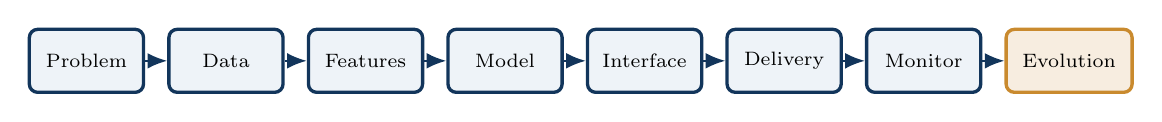
\begin{tikzpicture}[node distance=0.28cm]
  \node[flowbox, minimum width=1.45cm, minimum height=0.8cm] (problem) {\scriptsize Problem};
  \node[flowbox, minimum width=1.45cm, minimum height=0.8cm, right=of problem] (data) {\scriptsize Data};
  \node[flowbox, minimum width=1.45cm, minimum height=0.8cm, right=of data] (features) {\scriptsize Features};
  \node[flowbox, minimum width=1.45cm, minimum height=0.8cm, right=of features] (model) {\scriptsize Model};
  \node[flowbox, minimum width=1.45cm, minimum height=0.8cm, right=of model] (interface) {\scriptsize Interface};
  \node[flowbox, minimum width=1.45cm, minimum height=0.8cm, right=of interface] (delivery) {\scriptsize Delivery};
  \node[flowbox, minimum width=1.45cm, minimum height=0.8cm, right=of delivery] (monitor) {\scriptsize Monitor};
  \node[accentbox, minimum width=1.6cm, minimum height=0.8cm, right=of monitor] (evolution) {\scriptsize Evolution};
  \foreach \a/\b in {problem/data,data/features,features/model,model/interface,interface/delivery,delivery/monitor,monitor/evolution} {
    \draw[arrow] (\a) -- (\b);
  }
  \end{tikzpicture}

  \vspace{0.5em}
  \begin{block}{Today in the course}
  \textbf{Focus:} #1

  \textbf{Bridge:} #2
  \end{block}

  \begin{columns}[T]
  \column{0.48\textwidth}
  \begin{block}{Fraud case}
  {\footnotesize #3}
  \end{block}
  \column{0.48\textwidth}
  \begin{block}{Pasteurization case}
  {\footnotesize #4}
  \end{block}
  \end{columns}

  \vspace{0.3em}
  {\footnotesize \textbf{Course thread:} #5}
  \coursefooter
  \end{frame}
}

\newcommand{\classclosingframe}[4]{
  \begin{frame}{From This Class to the Next}
  \begin{block}{What stays with us}
  #1
  \end{block}

  \begin{columns}[T]
  \column{0.48\textwidth}
  \begin{block}{Project use}
  {\footnotesize #2}
  \end{block}
  \column{0.48\textwidth}
  \begin{block}{Next connection}
  {\footnotesize #3}
  \end{block}
  \end{columns}

  \vspace{0.3em}
  {\footnotesize \textbf{Course thread:} #4}
  \coursefooter
  \end{frame}
}

\tikzset{
  flowbox/.style={
    rounded corners=3pt,
    draw=courseblue,
    fill=courseice,
    very thick,
    minimum width=2.2cm,
    minimum height=0.9cm,
    align=center,
    font=\small
  },
  accentbox/.style={
    rounded corners=3pt,
    draw=coursegold,
    fill=coursegold!15,
    very thick,
    minimum width=2.2cm,
    minimum height=0.9cm,
    align=center,
    font=\small
  },
  arrow/.style={
    -{Latex[length=2.5mm,width=2mm]},
    thick,
    draw=courseblue
  }
}


\title{Class 32: Practical Project Brainstorm}
\subtitle{Session 32 of 36 -- Workshop: Choosing Your Capstone Idea}
\author{\coursename}
\date{}

\begin{document}

\frame{\titlepage \coursefooter}

\begin{frame}{Agenda}
\begin{itemize}
\item Why planning starts with a bounded idea, not just a good model
\item Defining problem, users, and scope
\item Objectives you can actually evaluate
\item Two project patterns from this repo, and how to propose your own
\item Idea screening checklist
\item Workshop deliverable: a one-page project pitch
\end{itemize}
\coursefooter
\end{frame}

\begin{frame}{Planning is part of the engineering work}
\learninggoals{
\begin{itemize}
\item Turn a vague ML idea into a bounded problem statement.
\item Distinguish MVP scope from stretch goals.
\item Screen a project idea against feasibility, data availability, and evaluability.
\item Leave this session with a one-page project pitch.
\end{itemize}
}
\coursefooter
\end{frame}

\coursecontextframe
{Choosing and scoping a capstone project idea.}
{This workshop turns the whole course arc, from Python and data-driven methods through MLOps, into the raw material for each team's own project.}
{The fraud case is used here as a worked example of a bounded, evaluable project pattern, not as a fixed assignment.}
{The pasteurization case is used the same way: a template for scope, not a required topic.}
{A good project idea is one you can already imagine requiring, testing, deploying, and monitoring, even before you have built any of it.}

\begin{frame}{Why planning matters in ML projects}
\begin{itemize}
\item ML systems evolve through data, code, models, interfaces, validation, and operations.
\item More roles means more handoffs, which means more need for shared artifacts.
\item A weak idea creates downstream confusion in requirements, evaluation, and release planning.
\end{itemize}
\begin{block}{Practical claim}
Planning does not remove uncertainty, but it makes uncertainty visible enough to manage.
\end{block}
\coursefooter
\end{frame}

\begin{frame}{A project summary defines boundaries}
\begin{itemize}
\item What problem is being solved?
\item Who uses or is affected by the result?
\item What is in scope for this project?
\item What is intentionally out of scope?
\item What evidence will convince stakeholders that the project is useful?
\end{itemize}
\coursefooter
\end{frame}

\begin{frame}{What a strong project summary should contain}
\begin{itemize}
\item Problem statement and target users.
\item Data sources and expected constraints.
\item Expected system output: prediction, forecast, alert, or recommendation.
\item Success criteria tied to technical and user outcomes.
\item Risks, assumptions, and dependencies.
\end{itemize}
\coursefooter
\end{frame}

\begin{frame}{Objectives should be specific enough to evaluate}
\begin{block}{Weak objective}
Build an ML system for quality control.
\end{block}
\begin{block}{Stronger objective}
Detect abnormal process trajectories from synthetic pasteurization sensor data and expose alerts through a dashboard with traceable event logs.
\end{block}
\begin{itemize}
\item Strong objectives are specific, measurable, relevant, and bounded enough to review.
\end{itemize}
\coursefooter
\end{frame}

\begin{frame}{Idea-generation prompts}
\begin{itemize}
\item What data do you already have access to, or can realistically get?
\item What decision would this system actually support, and for whom?
\item Who would be upset, or put at risk, if this system were confidently wrong?
\item Which part of the course lifecycle, data, model, interface, delivery, or monitoring, are you most curious to go deep on?
\end{itemize}
\coursefooter
\end{frame}

\begin{frame}{A more suitable proposal example}
\begin{block}{Project}
Forecast temperature and detect abnormal state transitions in a synthetic pasteurization line.
\end{block}
\begin{itemize}
\item Data source: Flask stream from `pasteurization/serving.py`.
\item MVP: predict next temperature value and visualize drift alerts.
\item Stretch goal: state-aware forecasting and alert triage.
\item Main risks: synthetic realism, label scarcity, and operator-facing thresholds.
\end{itemize}
\coursefooter
\end{frame}

\begin{frame}{Another project pattern students can defend}
\begin{block}{Project}
Fraud scoring as a service for transaction review support.
\end{block}
\begin{itemize}
\item Data source: credit-card fraud dataset and engineered features.
\item MVP: classify transactions and expose a scoring endpoint.
\item Stretch goal: threshold tuning plus analyst-facing dashboard.
\item Risks: class imbalance, false-positive cost, and drift after deployment.
\end{itemize}
\coursefooter
\end{frame}

\begin{frame}{Or propose your own, in the same shape}
\begin{itemize}
\item Data source: where does it come from, and can you actually access it this semester?
\item MVP: the smallest version that is still a complete pipeline, not just a model.
\item Stretch goal: the ambitious extension you would attempt only if the MVP lands early.
\item Main risks: name at least one data risk and one operational risk.
\end{itemize}
\coursefooter
\end{frame}

\begin{frame}{Idea screening checklist}
\begin{itemize}
\item Feasible: can this be built, at MVP scope, with the time and skills available?
\item Data-available: is there a realistic path to the data, not just a hope for it?
\item Evaluable: is there a way to say whether it worked?
\item Lifecycle-complete: can you sketch, even roughly, its requirements, a test, a deployment path, and a monitoring signal?
\end{itemize}
\begin{block}{Warning sign}
If you cannot answer one of these in one sentence, the idea is not ready to pitch yet.
\end{block}
\coursefooter
\end{frame}

\begin{frame}{Common brainstorm traps}
\begin{itemize}
\item Too big: the MVP is already a semester of work by itself.
\item Too vague: ``analyze the data and find insights'' has no defined output.
\item No data path: the idea depends on data nobody has confirmed access to.
\item Pure research question: interesting, but there is no system for anyone to use.
\end{itemize}
\coursefooter
\end{frame}

\begin{frame}{Inspiration already sitting in this repository}
\repoactivity{
\begin{itemize}
\item Notebooks and datasets used across the Python and data-driven blocks are fair game as a starting point, not only the two running cases.
\item `documents/FraudDetectionAsaService.pdf` and `documents/Forecasting_and_Drift_Pasteurization.pdf` show what a scoped project write-up looks like.
\item Reusing a case from class does not mean reusing the slides; it means reusing the data access and problem framing as a head start.
\end{itemize}
}
\coursefooter
\end{frame}

\begin{frame}{Discussion prompt}
\begin{block}{Question}
Swap your one-page pitch with another group. What is the first question you would ask them before agreeing this project is well scoped?
\end{block}
\begin{itemize}
\item This rehearses the kind of scrutiny a proposal review will apply later.
\item It also surfaces blind spots the original team stopped noticing.
\end{itemize}
\coursefooter
\end{frame}

\begin{frame}{Workshop deliverable: your one-page pitch}
\begin{itemize}
\item Problem and target users, in two sentences.
\item Data source and how you will access it.
\item MVP scope and one stretch goal.
\item Two named risks, one data-related and one operational.
\item One success criterion you could check by the end of the semester.
\end{itemize}
\coursefooter
\end{frame}

\begin{frame}{Papers and materials}
\readinglist{
\href{https://www.oreilly.com/library/view/designing-machine-learning/9781098107956/}{Designing Machine Learning Systems};\
\href{https://www.productplan.com/glossary/minimum-viable-product/}{Minimum Viable Product guide};\
\href{https://www.atlassian.com/agile/project-management/epics-stories-themes}{Project planning with epics and stories}.
}
\coursefooter
\end{frame}

\classclosingframe
{\begin{itemize}
\item A good project idea is bounded, evaluable, has a real data path, and touches the whole lifecycle.
\item MVP and stretch goals should be written down separately from the start.
\item Screening an idea against a short checklist catches most scoping mistakes early.
\end{itemize}}
{Keep your one-page pitch; it is the direct input to the development plan built in Class 34.}
{Class 33 brings in a guest speaker, Sbroiavacca, as a real-world bridge right before Class 34 turns your pitch into milestones and a development plan.}
{Today's pitch is the first draft of the project that will carry through requirements, delivery, and monitoring for the rest of the course.}

\end{document}
